\chapter{Porównanie testowalności na przykładzie aplikacji}
\label{analiza_testow}

\section{Opis doświadczenia}
\textit{---------draft-------------}

Na przykładzie jednej z aplikacji postaram się przedstawić różnicę w podejściu do testowania w przypadku programu dla systemu Android napisanego w architekturze „standardowej” i tego samego programu napisanego przy użyciu Clean Architecture.

Do tego celu autor wykorzysta aplikację \textit{JSON Web Token Authentication for Android} napisaną przez Victora Albertosa , a której źródła udostępnione są w serwisie GitHub na licencji \textit{open source}. 

https://github.com/VictorAlbertos/RestAPIParseAuthAndroid

https://github.com/VictorAlbertos/RestAPIParseAuthCleanAndroid

\section{Opis aplikacji}
\textit{---------draft-------------}

Uwierzytelnianie dla Androida i iOS. 

Aplikacja służy do autentykacji użytkowników Androida i iOS korzystając z \textit{REST API} serwera \textit{Parse} oraz textit{JSON\footnote{JSON, JavaScript Object Notation – lekki format wymiany danych komputerowych. JSON jest formatem tekstowym, bazującym na podzbiorze języka JavaScript. Źródło: Wikipedia.} Web Tokens (JWT)}. JWT to otwarta, według standardu przemysłowego RFC 7519\cite{website:jwt:rfc7519}, metoda do uwierzytelniania stron w środowisku aplikacji internetowych. Wykorzystywana jest do przekazywania tożsamości użytkowników między dostawcą, a odbiorcą usług internetowych lub innego typu uwierzytelnień zgodnie z logiką biznesową. Tokeny mogą także być uwierzytelniane i szyfrowane. 

Serwer \textit{Parse} to wspólna platforma do przechowywania danych i interakcji z usługami internetowymi dla aplikacji mobilnych. Wielu programistów decyduje się na wykorzystanie tej platformy, zamiast pisać własne rozwiązania w tym zakresie.

Victor Albertos zdecydował się użyć wyżej wymienionego rozwiązania, aby zwiększyć pielęgnowalność aplikacji: móc modyfikować logikę biznesową nie modyfikując aplikacji po stronie klienta. Serwer Parse, jako rozwiązanie uniwersalne, zapewniał takie podejście \cite{website:victor:application}.

\section{Zasada działania}
\textit{---------draft-------------}

Użytkownik loguje się za pomocą swojej nazwy użytkownika i hasła do serwera Parse. Jeżeli nie ma jeszcze konta na serwerze, za pomocą aplikacji może je sobie założyć. Od chwili zalogowania może korzystać z przeznaczonych mu usług serwera, logując się z wielu urządzeń i otwierając wiele sesji.

\section{Analiza aplikacji pod względem testowalności}

\subsection{Budowa aplikacji w architekturze standardowej}
\textit{---------draft-------------}
Autor skupia się na budowie aplikacji tylko z punktu widzenia testowania aplikacji.

\begin{figure}[!htb]
    \centering
    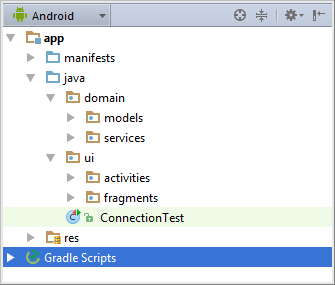
\includegraphics[width=10cm]{imgs/ch6_app_st.png}
    \caption
{Schemat budowy aplikacji w architekturze standardowej}
    \label{fig:app_std}
\end{figure} 


\subsection{Budowa aplikacji wykorzystując \textit{Clean Architecture}}
\textit{---------draft-------------}

Każde z wymienionych w poprzednim rozdziale podejść do uporządkowania architektury systemowej można wykorzystać do polepszenia testowalności aplikacji tworzonych dla tego systemu. Analizując je krok po kroku można dojść do wniosku, że ich idea jest taka sama, a różnią się szczegółami. Dla celów tej pracy wystarczy wybrać jedną z nich - w tym przypadku autor zdecydował się na \textit{The Clean Architecture}, opisaną w rozdziale \ref{clean_architecture_opis}.

\begin{figure}[!htb]
    \centering
    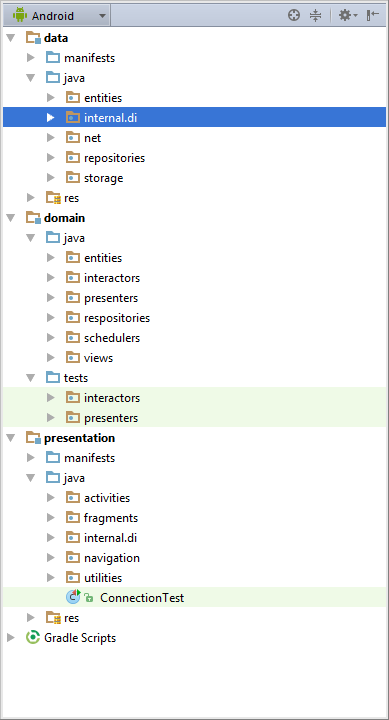
\includegraphics[width=10cm]{imgs/ch6_app_cl.png}
    \caption
{Schemat budowy aplikacji w \textit{Clean Architecture}}
    \label{fig:app_std}
\end{figure} 


\section{Przebieg doświadczenia}
\textit{---------draft-------------}

Przeprowadzono testy osobno dla obu projektów, wykorzystując to samo środowisko Android Studio w wersji 1.5.1, ten sam komputer i ten sam emulator: Nexus\_5\_API\_23.

\newpage
\section{Wyniki doświadczenia}
\label{wyniki_doswiadczenia}
\subsection{Architektura standardowa}
\textit{---------draft-------------}

\begin{itemize}
\item
Brak testów jednostkowych. Brak weryfikacji błędów w kodzie na bieżąco. Patrz rysunek \ref{fig:odwrocona_piramida}.

\begin{figure}[!htb]
    \centering
    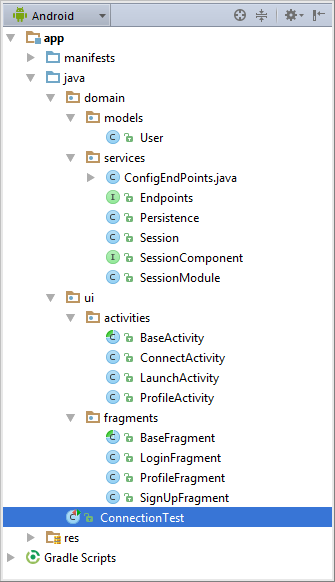
\includegraphics[width=10cm]{imgs/ch6_app_st_test1.png}
    \caption
{Brak testów jednostkowych. jedynym dostępnym jest test integracyjny.}
    \label{fig:app_std_test1}
\end{figure} 


\item
Jedynym testem jest \textit{ConnectionTest}. Czas trwania: 241s. Wymaga uruchomienia emulatora bądź podłączenia fizycznego urządzenia. W przypadku błędu w kodzie testy wydłużają się, gdyż za każdym razem trzeba uruchomić \textit{ConnectionTest}.
Wynik testu przedstawia rysunek \ref{fig:app_std_test2}

\begin{figure}[!htb]
    \centering
    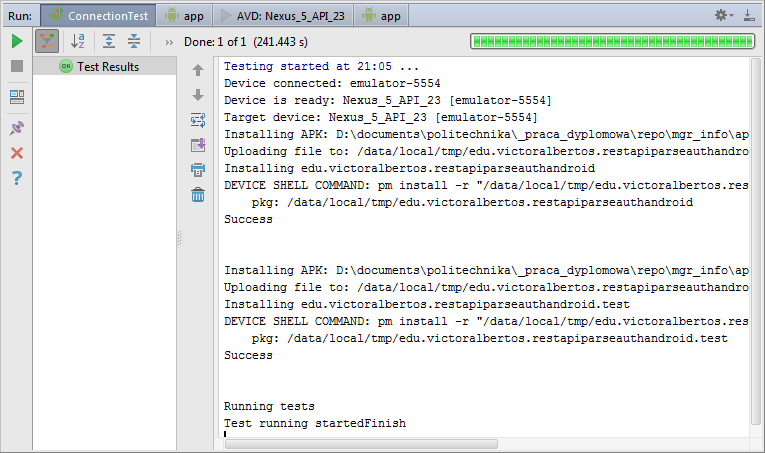
\includegraphics[width=15cm]{imgs/ch6_app_st_test2.png}
    \caption
{Wynik testu integracyjnego. Długi czas trwania.}
    \label{fig:app_std_test2}
\end{figure} 

\end{itemize}

\newpage
\subsection{\textit{Clean Architecture}}
\textit{---------draft-------------}

\begin{itemize}
\item
Tutaj są zarówno testy jednostkowe jak i test integracyjny \textit{ConnectionTest}.

Strukturę testów jednostkowych przedstawia rysunek \ref{fig:app_cl_test1}
\begin{figure}[!htb]
    \centering
    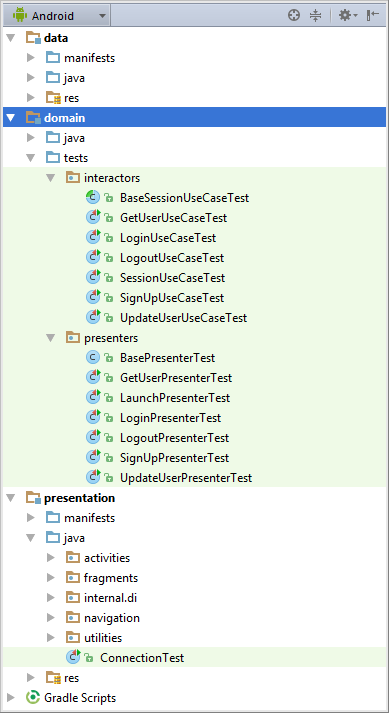
\includegraphics[width=10cm]{imgs/ch6_app_cl_test1.png}
    \caption
{Struktura testów jednostkowych}
    \label{fig:app_cl_test1}
\end{figure} 

\item
Wyniki testów jednostkowych przedstawiają rysunki \ref{fig:app_cl_test5}, \ref{fig:app_cl_test3} i \ref{fig:app_cl_test4}.

\begin{figure}[!htb]
    \centering
    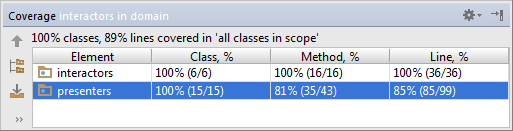
\includegraphics[width=12cm]{imgs/ch6_app_cl_test5.png}
    \caption
{Wyniki wraz z pokryciem kodu}
    \label{fig:app_cl_test5}
\end{figure} 

\begin{figure}[!htb]
    \centering
    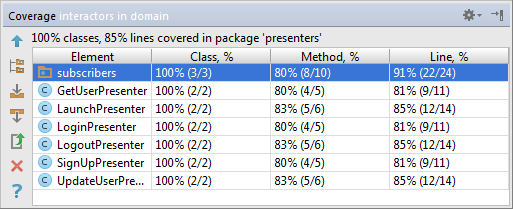
\includegraphics[width=12cm]{imgs/ch6_app_cl_test3.png}
    \caption
{Wyniki wraz z pokryciem kodu}
    \label{fig:app_cl_test3}
\end{figure} 

\begin{figure}[!htb]
    \centering
    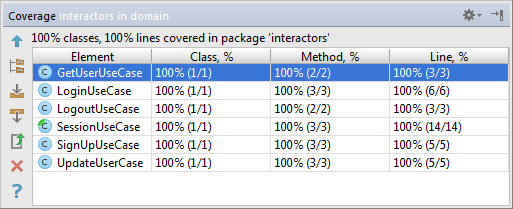
\includegraphics[width=12cm]{imgs/ch6_app_cl_test4.png}
    \caption
{Wyniki wraz z pokryciem kodu}
    \label{fig:app_cl_test4}
\end{figure} 

\item
Test integracyjny również jest szybszy i trwa 167s. Wynik przedstawiony na rysunku \ref{fig:app_cl_test6}

\begin{figure}[!htb]
    \centering
    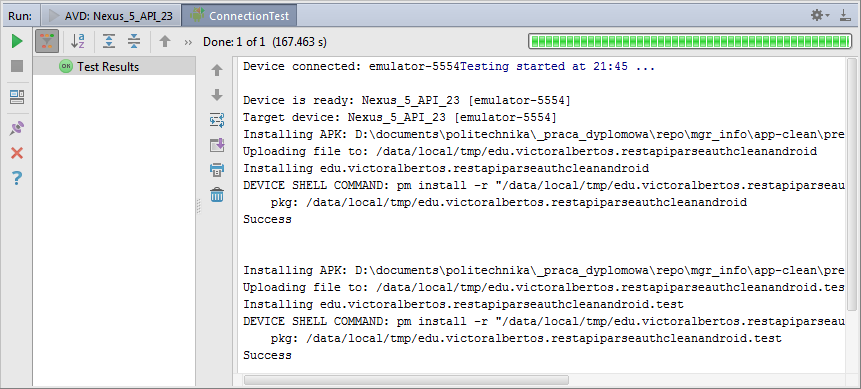
\includegraphics[width=15cm]{imgs/ch6_app_cl_test6.png}
    \caption
{Wynik testu integracyjnego}
    \label{fig:app_cl_test6}
\end{figure} 

\end{itemize}
